\documentclass[a4paper, 12pt]{article}
\usepackage{graphicx}
\usepackage[T1]{fontenc}
\usepackage[utf8]{inputenc}
\usepackage{tabularx,ragged2e,booktabs}
\usepackage{caption}
\usepackage{subcaption}
\usepackage{float}
\usepackage{url}
\usepackage{enumerate}
\usepackage{amsmath}
\usepackage{amssymb}
\usepackage{alltt}
\usepackage{listings}
\usepackage{pdfcolparallel}
\usepackage{scrextend}
\usepackage{wrapfig}
\usepackage{mathtools}
\usepackage [english]{babel}
\usepackage{array}
\usepackage{indentfirst}
\usepackage[letterpaper]{geometry}
\usepackage{times}
\geometry{top=0.8in, bottom=0.8in, left=0.9in, right=0.9in}

\lstset{
  basicstyle=\ttfamily,
  mathescape
}



\newcommand{\tab}[1]{\hspace{.2\textwidth}\rlap{#1}}

\begin{document}
\begin{titlepage}
	\centering
    \rule{\textwidth}{1pt}

	\vspace{0.5cm}
	{\Huge\bfseries The Application of Reinforcement Learning Algorithms to Popular Web Games\par}
   	\vspace{0.5cm}
    \rule{\textwidth}{1pt}

    \vspace{1cm}
    {\Large\itshape Contributors\par}
    {Elliot Shohet, Michael Mathew, Grigor Ambartsumyan,

    Anmol Singh, Ibrahim Ahmed, Tuan Vu, Haoyao Chen,

    Inka Arifin, Guranjan Singh, Ronil Singh,

    Masayuki Takagi, Ahsan Abdullah

	}



	\vfill
% Bottom of the page
	Professor\par
	\textsc{Ilias Tagkopoulos}

	{\today\par}
\end{titlepage}

\section*{Abstract}

Decision making is an essential attribute of any intelligent agent. In this project, we addressed the problem of teaching an agent to learn the optimal policy for a given state. In context of the web games presented below, we taught both the doodle in Doodle Jump, and the bird in Flappy Bird, a set of moves that maximized their respective long-term cumulative score (a.k.a. reward) by utilizing the subset of Machine Learning algorithms known as Reinforcement Learning. We explicitly defined the three main components of a reinforcement learning algorithm - the state set, the action set, and the rewards - in such a manner that convergence was relatively quick, and performance was above that of a skilled player.

Our results indicate that there exists a trade-off between the granularity captured by the  state set and how long it takes until the algorithm performs well. In Doodle Jump, a much smaller state set resulted in faster learning, but lower absolute scores when compared to a higher granularity variant (avg score of 8000 vs 23000). High granularity variants performed well in the long-run, but took significantly longer to train and required more resources in order for the algorithm to work.

By open-sourcing our projects and this report$^{[8]}$$^{[9]}$, we hope that we can improve the effectiveness of Reinforcement Learning algorithms in fully-fledged and modern web games with non-trivial state-action sets.

\section{Introduction}
In other Supervised Learning algorithms specific samples with explicit labels are given as input with the objective of recognizing patterns within the data to provide a meaningful output (Artificial Neural Networks, Support Vector Machines, Naive Bayes, etc). However, in Reinforcement Learning, there is no predefined correct output to a specific input, but rather there exists an agent that learns the best possible output for a given state through trial and error.$^{[1]}$

A game is a simple and efficient way to see the effects of Reinforcement Learning. In most  games, an agent, ideally, performs an action in a given state that increases its long-term score, where the states are defined as a combination of any factors that affect the agent's decision.$^{[3]}$ As the agent explores the state set, it rewards actions that increase its score and penalizes actions that don't, thus allowing the agent to "learn".

The problem of building intelligent agents in games has been addressed by many algorithms in the past. For example, Deep Convolution Networks have learned how to play Go$^{[7]}$, and Deep Q Networks have learned how to play over 49 classic Atari Games to the same level as professional human game testers$^{[8]}$. However, not a whole lot of progress has been made towards applying reinforcement learning algorithms to popular and modern web games. While the implementations referenced above are important, a novice machine learning enthusiast would more likely benefit from seeing how to apply reinforcement learning algorithms to modernly-implemented web games, which have been gaining popularity over their desktop application counterparts recently.

In this paper, and in the open source code we've published on Github, we show an effective implementation of the reinforcement learning algorithm called Q-Learning to Doodle Jump, after being inspired by the performance of the same algorithm applied to Flappy Bird, a much simpler, but still immensely popular game$^{[4]}$. We also introduce new factors to the both games: granularity/resolution, exploration, decision frequency, and tick frequency, which help reduce the amount of time it takes for the algorithm to perform well. A combination of the new and old hyperparameters of Q-Learning show scores of over 30,000 (in DJ) - well above that of a skilled player - in a relatively short amount of time without much computation power.

\par


\section{Methods}


\subsection{Flappy Bird}

\subsubsection{Q-Learning Algorithm $^{[4]}$}

\begin{Parallel}{0.49\textwidth}{0.49\textwidth}
\ParallelLText{
    \textbf{Inputs:}
    \begin{itemize}
        \item S is a set of states
        \item A is a set of actions
        \item $\gamma$ the discount factor
        \item $\alpha$ the step size
    \end{itemize}
}
\ParallelRText{
    \textbf{Local:}
    \begin{itemize}
        \item Real array of Q[s,a]
        \item Previous state s
        \item Previous action a
    \end{itemize}
    }
\ParallelPar
\end{Parallel}

% Do we really need the pseudocode if we're explaining learning below?
\begin{lstlisting}

  Pseudocode:
  Initialize Q[s,a] arbitrarily
  Observe the current state s
  Repeat
    Select and carry out and action a
    Observe reward r and state s'
    Q[s, a] $\leftarrow$ Q[s, a] + $\alpha$(r + $\gamma\:max_{a}$ Q[s', a'] - Q[s, a])
    s $\leftarrow$ s' until termination
\end{lstlisting}

\begin{center}\(Q(s,a) = Q(s,a) + \alpha (reward +  \gamma Q(s',a') - Q(s,a))\)\end{center}

\subsubsection{Application of Q-Learning to Flappy Bird}

The application of Q-Learning to Flappy Bird is training an agent, the bird, to perform an optimal action in any state. In order to accomplish this, the agent explores a state set and assigns rewards based off of whether an action from one state produced a favorable outcome.$^{[3]}$ Q-Learning, in particular, is a model free form of reinforcement learning.$^{[5]}$ This means, the agent must interact with its environment directly to obtain information.\\

\noindent\textbf{Learning:}
The array Q is initialized with zeros. Every time we reach a state, denoted by \textit{s}, we choose the best action (the action that will maximize the expected reward). In the case of a tie, we "Do Nothing."
    \begin{enumerate}
    \setlength{\itemsep}{0.2pt}
    \item Observe the state s and perform the action \textit{max Q[s,a]} that maximizes the reward. On the next tick of the game engine, the agent is now in the next state s'.
    \item Observe the new state, \textit{s'} and the reward that is associated with it. If the bird is still alive +1, otherwise -1000.
    \item Update the Q array according to the rule we defined in section 2.1.1.
    \item Set the current state to \textit{s'} and repeat the loop.
    \end{enumerate}

\subsubsection{State Set Reduction}

\setlength{\columnsep}{18pt}
\begin{wrapfigure}{r}{0.25\textwidth}
    \centering
	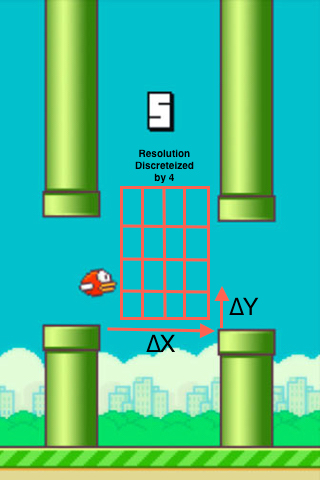
\includegraphics[width=5.5cm]{FlappyBirdStateSet.jpg}
\end{wrapfigure}

The state set is defined by the vertical distance from the next lower pipe to the bird, $\Delta$Y, and the horizontal distance from the next pipe to the bird, $\Delta$X. Due to the continuous nature of the state set, There is a division to both the vertical and horizontal distances called the \textit{resolution/granularity} factor. This means that the result is rounded to the nearest integer to make the state set discrete and small.

\subsubsection{Reward Process}

The agent was given a reward at every tick, which occurs at the rendering of each frame. If the agent died as a result of their choice, we assigned the action selected a reward of -1000. If the agent lived, we assigned a small reward of 1. By doing the aforementioned, we effectively penalized deaths, resulting in the agent learning how to maximize its life, and therefore its score.

\subsubsection{Action Process}

In this game, the agent can only perform two actions in any given state: jump up or do nothing and begin to fall.

\subsection{Doodle Jump}

\subsubsection{Parameters}
\begin{itemize}
	\setlength{\itemsep}{0.2pt}
	\item \textit{xdivision, ydivision}: Round distance to the nearest division
    \item \textit{brain.learning\_rate}: Scales how fast the predicted rewards change
    \item \textit{scale\_death}: Adjusts the penalty for death at higher scores
    \item \textit{decision}: The y velocity at which a decision is made
\end{itemize}
\subsubsection{Local Variables}
\textit{previous score,    previous collision,    target platform,    last state}: info from last decision


\textit{actions:} The cumulative reward for going to each platform


\textit{explored:} The number of unique states encountered


% \begin{itemize}
% 	\setlength{\itemsep}{0.4pt}
%     \item \textit{previous\_score}: The score at the previous decision point
%     \item \textit{previous\_collision}: The platform that the doodle landed on previously
%     \item \textit{target\_platform}: The currently selected platform to land on
%     \item \textit{brain.actions}: The cumulative reward for going to each platform
%     \item \textit{brain.explored}: The number of unique states encountered
%     \item \textit{brain.last\_state}: The last predicted state, used for updating rewards
% \end{itemize}

\subsubsection{Implementation}
	\begin{enumerate}
    	\item The "brain" of the agent is a 3-dimensional array of cumulative rewards indexed by the state of each on screen platform.
        \item The states are a 3-tuple of platform type, y-distance, and x-distance. The state space for our model is 2,580.
        	\begin{enumerate}
            	\item Platform type takes on the value of 0 for solid platforms, 1 for broken platforms, and 2 for moving platforms.
                \item Y-distance is the vertical distance between the player and the platform ranging from -550 to 310, rounded to the nearest \textit{ydivision}. This distance is relative as it is important to know if the platform is above or below.
                \item X-distance is the horizontal distance between the player and the platform ranging from 0 to 400, rounded to the nearest \textit{xdivision}. This distance is absolute as the direction does not affect the possibility of landing on it.
            \end{enumerate}
    \end{enumerate}
\subsubsection{State Set Reduction}
Using floating point for the position of the platforms and the player would result in over 1 billion possible states. Thus, it was important to reduce the dimensionality of the problem. The x distance and y distance are rounded to integers. However, simply rounding to the nearest integer would still result in over a million states. The parameters \textit{xdivision} and \textit{ydivision} are used to round the distances into a small set of discrete values. Larger divisions result in a smaller state set and decreased accuracy. Through trial and error, it was determined that the values \textit{xdivision} = 40 and \textit{ydivision} = 10 resulted in a sufficient compromise between model complexity and accuracy. The platform height is 17, the width is 70, so these values provide sufficient overlap and granularity. \textit{Figure 1} shows the effect of \textit{xdivision} and \textit{ydivision}. \textit{Figure 1a} shows two platforms that would be recognized as different states in our model. \textit{Figures 1b-d} show pairs of platforms that would be recognized as the same state in our model. With lower division values, these could be distinguished at the cost of increased complexity, training time, and computing requirements.
\begin{figure}[H]
\centering
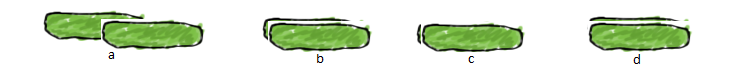
\includegraphics[scale=0.75]{platform_overlap.png}
\caption{Platform Granularity}
\end{figure}

\subsubsection{Decision Process}
\begin{enumerate}
	\setlength{\itemsep}{0.2pt}
	\item At a predetermined agent velocity, set by the variable \textit{decision}, read in all possible next states.
    	\begin{enumerate}
        	\setlength{\itemsep}{0.2pt}
        	\item If the state has been seen before, then it exists within the brain object.
            \item If the state has never been seen before, add the state to the brain object and initialize its reward to a random number from 1 to 100.

        \end{enumerate}
    \item Pick the platform with the maximum reward based on the value indexed by a state in the brain object.
    \item Assign this as the target platform, then move towards it.
\end{enumerate}
\subsubsection{Reward Process}
\begin{enumerate}
\setlength{\itemsep}{0.2pt}
\item If the agent moves towards the target platform and dies, penalize that platform's state by a fixed amount.
\item If the agent moves towards the target platform and successfully lands on it, reward that target platform with the increase in score.
\item If the agent moves to the target platform, but does not successfully land on it and also does not die, then reward the platform the agent landed on with the increase in score and penalize the target platform by a fixed amount. Penalizing the missed platform causes the doodle to change its decision if it gets stuck.
\end{enumerate}

\section{Results}
\subsection{Flappy Bird}

\subsubsection{$\alpha$, the Learning Rate}

\begin{figure}[H]

\centering
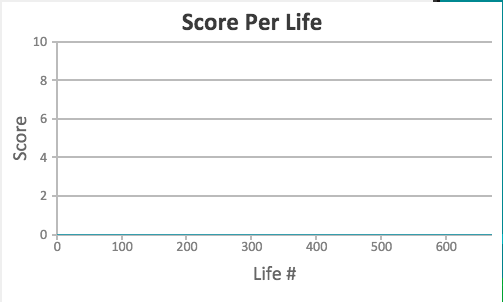
\includegraphics[width=.3\textwidth]{alpha0_0.png}\hfill
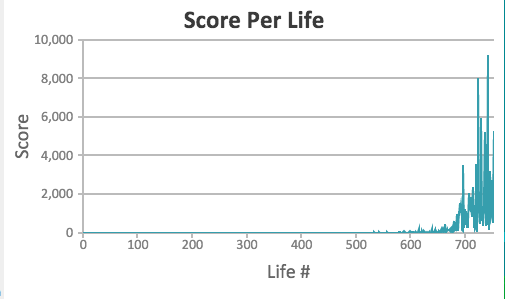
\includegraphics[width=.3\textwidth]{alpha0_2.png}\hfill
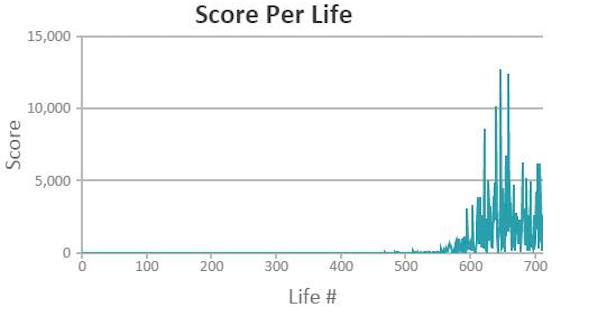
\includegraphics[width=.3\textwidth]{alpha0_6.png}\hfill
\caption{X axis = trials, Y axis = scores. From left to right, $\alpha$ = 0, 0.2, 0.6.}

\end{figure}


\subsubsection{Resolution/Granularity, the State Set Size Divider}


    \begin{figure}[H]
    \centering
    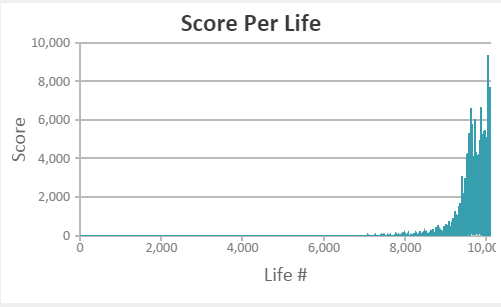
\includegraphics[width=.3\textwidth]{A0_7_R01_E00.png}\hfill
    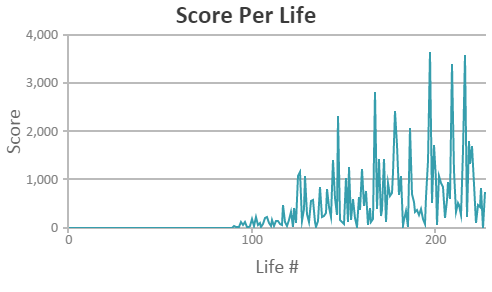
\includegraphics[width=.3\textwidth]{Overnight_Alpha_0_7_-_Res_10_-_Explor_0_0_GRAPH.PNG}\hfill
    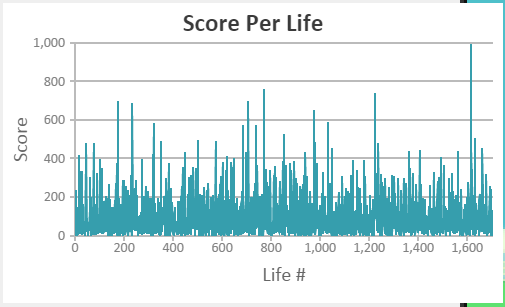
\includegraphics[width=.3\textwidth]{A0_7_R100_E00_Var1.png}\hfill
    \caption{X axis = trials, Y axis = the scores. From left to right, resolution = 1, 10, 100.}
    \end{figure}

\subsubsection{$\epsilon$, the Exploration Rate}


\begin{figure}[H]

\centering
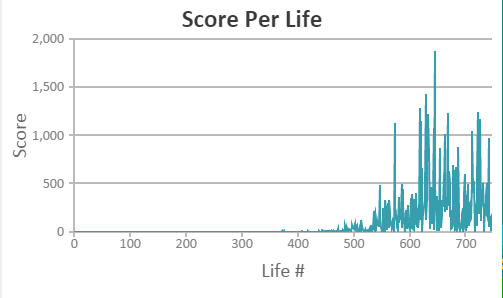
\includegraphics[width=.3\textwidth]{0_7-4-0-score.png}\hfill
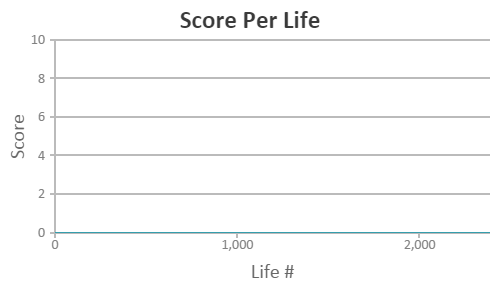
\includegraphics[width=.3\textwidth]{0_7-4-0_4-score.png}\hfill
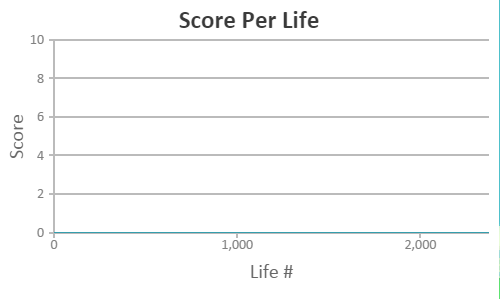
\includegraphics[width=.3\textwidth]{0_7-4-0_8-score.png}\hfill
\caption{X axis = trials, Y axis = the scores. From left to right, $\epsilon$ = 0, 0.4, 0.8.}

\end{figure}
\subsubsection{$\gamma$, the Discount Rate}

\begin{figure}[H]

\centering
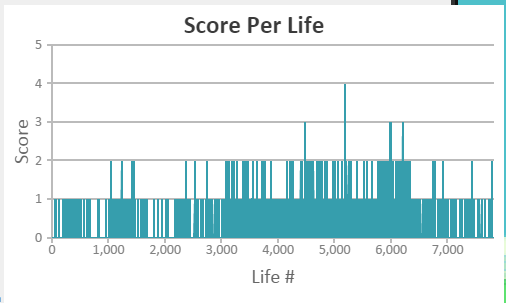
\includegraphics[width=.3\textwidth]{A0_7_R4_E0_G0.png}\hfill
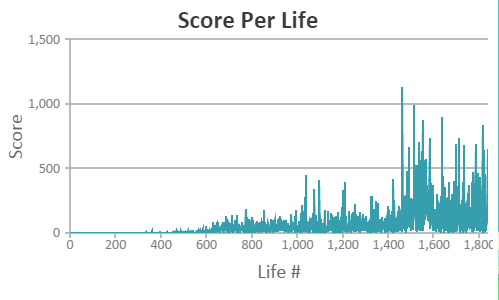
\includegraphics[width=.3\textwidth]{0_7-4-0-0_4-score.png}\hfill
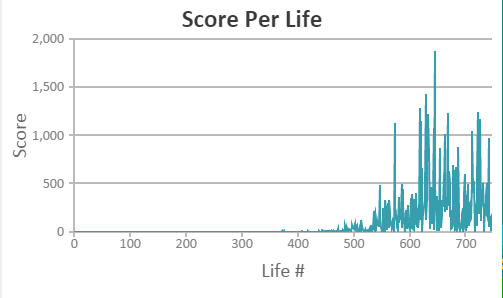
\includegraphics[width=.3\textwidth]{0_7-4-0-score.png}\hfill

\caption{X axis = trials, Y axis = the scores. From left to right, $\gamma$ = 0, 0.4, 1.}
\end{figure}

\subsection{Doodle Jump}
\begin{table}[H]
\caption{Varying Granularity}
\centering
\scalebox{0.75}{
\begin{tabular}{|l|c|c|c|l|l|l|}
\hline
\textbf{X Division} & 8 & 20 & 40 & 60 & 80 & 100 \\ \hline
\textbf{Y Division} & 2 & 5 & 10 & 15 & 20 & 25 \\ \hline
\textbf{Learning Rate} & 1 & 1 & 1 & 1 & 1 & 1 \\ \hline
\textbf{Avg Score} & 5000 & 23000 & 12000 & 15000 & 28000 & 8000 \\ \hline
\textbf{States Explored} & \multicolumn{1}{l|}{22902} & \multicolumn{1}{l|}{5389} & \multicolumn{1}{l|}{1745} & 947 & 600 & 419 \\ \hline
\textbf{Total States} & \multicolumn{1}{l|}{64500} & \multicolumn{1}{l|}{10320} & \multicolumn{1}{l|}{2580} & 1148 & 644 & 426 \\ \hline
\textbf{States Explored \%} & \multicolumn{1}{l|}{35.51} & \multicolumn{1}{l|}{52.22} & \multicolumn{1}{l|}{67.64} & 82.49 & 93.17 & 98.36 \\ \hline
\end{tabular}}
\end{table}

\begin{table}[H]
\centering
\caption{Varying Learning Rate}
\scalebox{0.75}{
\begin{tabular}{|l|c|c|c|l|l|l|}
\hline
\textbf{X Division} & 40 & 40 & 40 & 40 & 40 & 40 \\ \hline
\textbf{Y Division} & 10 & 10 & 10 & 10 & 10 & 10 \\ \hline
\textbf{Learning Rate} & 0.1 & 0.25 & 0.5 & 0.75 & 0.9 & 1 \\ \hline
\textbf{Avg Score} & 16000 & 13000 & 15000 & 11000 & 10000 & 12000 \\ \hline
\textbf{States Explored} & \multicolumn{1}{l|}{1745} & \multicolumn{1}{l|}{1733} & \multicolumn{1}{l|}{1746} & 1741 & 1719 & 1745 \\ \hline
\textbf{Total States} & \multicolumn{1}{l|}{2580} & \multicolumn{1}{l|}{2580} & \multicolumn{1}{l|}{2580} & 2580 & 2580 & 2580 \\ \hline
\textbf{States Explored  \%} & \multicolumn{1}{l|}{67.64} & \multicolumn{1}{l|}{67.17} & \multicolumn{1}{l|}{67.67} & 67.48 & 66.63 & 67.64 \\ \hline
\end{tabular}}
\end{table}

% \subsubsection{Notable Results}

    \begin{figure}[H]
\centering
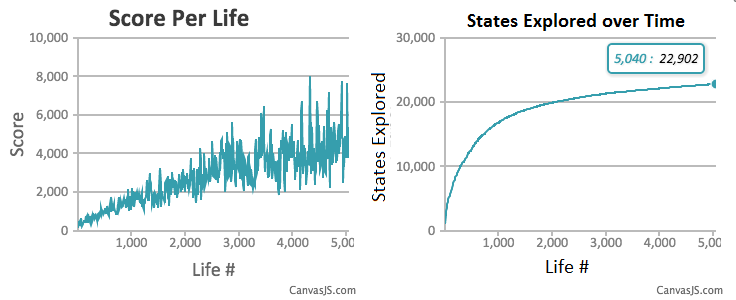
\includegraphics[scale=0.6]{x8_y2_rate1.png}
\caption{\textit{xdivision} = 8, \textit{ydivision} = 2, \textit{learning rate} = 1}
\end{figure}

\begin{figure}[H]
\centering
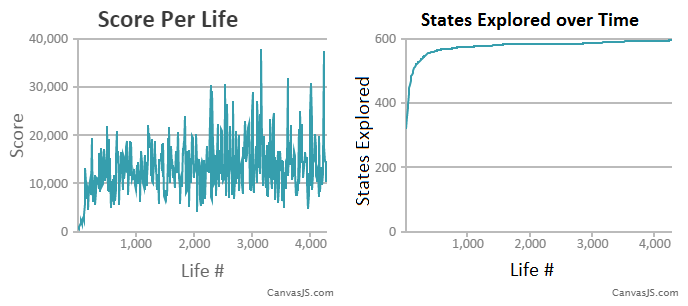
\includegraphics[scale=0.6]{x80_y20_rate1.png}
\caption{\textit{xdivision} = 80, \textit{ydivision} = 20, \textit{learning rate} = 1}
\end{figure}

    \begin{figure}[H]
\centering
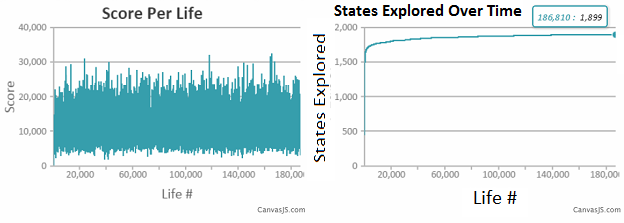
\includegraphics[scale=0.6]{x40y10rate1.png}
\caption{\textit{xdivision} = 40, \textit{ydivision} = 10, \textit{learning rate} = 1}
\end{figure}



\section{Discussion}
\subsection{Flappy Bird}

We sped up the tick rate of the game in order to reduce the amount of time it took to converge from 6-7 hours down to 15 minutes. Additionally, all four of the algorithm's hyper-parameters were exposed for the user to adjust and gather data. Different combinations of these parameters, $\alpha$, \textit{Resolution/Granularity}, \textit{Exploration Rate $\epsilon$}, and the Discount Rate $\gamma$, produced the results itemized in the following subsections. Certain combinations of these parameters produced satisfactory results, often yielding scores over 9000.

\subsubsection{Varying $\alpha$, the Learning Rate}

With alpha set to 0 and the rest of the variables constant, the score was constantly zero. At $\alpha$ = 0.2 the bird starts increasing its score after the 600\textsuperscript{th} trial, scoring ~8000 after the 700\textsuperscript{th} iteration. With $\alpha$ = 0.6, the score starts increasing significantly after the 500\textsuperscript{th} iteration, reaching well above 10000 around the 650\textsuperscript{th} iteration.

This observation makes sense since the learning rate is essentially how much of the newly discovered information is actually stored. Typically we'd start with a high learning rate, which allows fast changes, and then we'd slowly decrease it as time progresses. $^{[10]}$ So, when $\alpha$ was 0, it never retained any new information it learned, thus its score was stuck at zero. This coincides with what we'd find we if set $\alpha$ to 0 in the Q-Learning equation presented in 2.1.1.
%"update rule of Q-Learning algorithm" rather than Q-Learning Equation?
%"So, when alpha was 0, it never" it here sounds confusing?
\subsubsection{Varying Resolution/Granularity, the State Set Divider}

The value of resolution is significant in that it decides the size of the state set. The $floor()$ function is utilized to help us divide the game screen into discretized states. In our 540 x 180 pixel screen, if resolution is set to 10, the size of the state set would be determined as follows: $floor(540 / 10) = 54$; $floor(180/10) = 18$. The size of the state set is therefore 54-by-18. The higher the resolution, the smaller the state set, and vice-versa. A larger state set results in more accuracy at the expense of additional training time and computational resources. A smaller state set takes less time to train, but results in less accurate decisions being made since, in this particular case, states are grouped together with adjacent states.

By setting $\alpha$ to 0.7, Exploration Rate to 0, $\gamma$ to 1, and letting the the Resolution divider vary, we show the balance between accuracy and performance in section 3.1.2. We found that when $Resolution = 1$, the Q-Learning algorithm learns very slowly and only gains any sort of score after approximately 7000 deaths; however, it reaches a maximum score around 10,000. When $Resolution = 10$, it starts to make intelligent decisions after approximately a couple hundred deaths and reached a maximum score around 4000. When $Resolution = 100$, the algorithm gained score as soon as it began but it only can reach a maximum score of less than 1000.

\subsubsection{Varying $\epsilon$, the Exploration Rate}


In the context of Q-Learning, the Exploration Rate determines the "willingness" of the algorithm to try a random action, completely ignoring what it's learned, in hopes that this random action will result in better long-term performance. When the exploration rate is set to zero, the bird is conservative and always picks the best known action for the given state. However, given that there are only two actions that can be taken in any state(up, down/do nothing), any relatively high value for exploration rate would prevent the bird from truly learning. A random action taken in such an instance is binary and is thus not complex enough to truly utilize the randomness of the exploration rate. This becomes very apparent in the other two figures provided in 3.1.3 of the results section. With exploration rate set equal to 0.4 and 0.8, the bird does not learn at all with an average score of zero.

\subsubsection{Varying $\gamma$, the Discount Factor}

The discount rate determines whether there is more emphasis on the current reward compared to future rewards. The results of the score per life plots convey that the higher the $\gamma$, the higher the score. From the graphs in section 3.1.4, we can see that for $\gamma$ equal to 0, the highest score for over 7,000 trials was only 4. On the other hand, for $\gamma$ equal to one, we reached the high score of roughly 1700 by the 700\textsuperscript{th} trial. For an intermediate value of $\gamma$ equal to 0.4, the highest score of roughly 1,200 was not reached until the 1,500\textsuperscript{th} trial. Therefore, we can conclude that not only does a higher $\gamma$ result in a higher score, but that it also reaches the higher score much faster. In other words, it learns better in this particular game.

Our results coincide with the game engine of the Flappy Bird and the Q-Learning algorithm presented in 2.1.1. Since we force our agent to select the best action after each frame is rendered, our agent must heavily weigh long-term rewards over short-term ones. This is due to the large iteration gap between when a decision is made, and how it actually affects the agent in the long run, hence why our results show that a higher $\gamma$ performs better than a lower one.

\subsubsection{Summary of Results}

We have found, empirically, that a good hyper-parameter variant for Flappy Bird is one with an $\alpha$ near 1, a small state set divider, an exploration factor that starts at 1 and quickly goes down to 0, and a $\gamma$ near 1.

\subsection{Doodle Jump}
\subsubsection{Division Granularity}
	The results for each of the experimental models were compared after 5,000 iterations (\textit{Table 1}). Varying the division sizes for $x$ and $y$ distances resulted in a change to the total number of states. An increase in division size results in a lower number of total states, and a decrease in division size results in a higher number of total states. Therefore, reducing division sizes resulted in less states being explored in the same amount of time. This also introduced states that would never be explored, because the game has a minimum and maximum y-distances between platforms.
\subsubsection{Learning Rate}
	The experimental models used for learning rate were compared in the same manner as the experimental models for division granularity. The models had similar exploration rates. Lower learning rates resulted in larger scores because the agent was able to explore more options before the weight of other options grew. With a large learning rate, the agent quickly learns a few good options, and is less likely to explore other candidates.
\subsubsection{Summary of Results}
	\textit{Figure 6} shows that with more divisions, it takes more time and space to train the model. Training this model to convergence would likely result in a slight increase in score. However, given computational and time constrains, the (40,10,1) model used in \textit{Figure 8} provides adequate accuracy while taking much less time and space to converge. With the (40,10,1) model, the majority of states are discovered in the first 5000 lives. The average score also does not change after this point.

\section{Conclusion}

In this project we demonstrated the application of Q-Learning to popular web games Flappy Bird and Doodle Jump. We have described, in detail, the precise methodology implemented to teach the agents the optimal set of actions that maximize their respective cumulative score. Experimenting with different combinations of hyper-parameters, we have found that the size of the state set really determines both how well the algorithm performs, how long it takes until the algorithm performs well, and whether or not it will even converge given the resources available to the algorithm. With a significantly reduced state-action set, we have achieved results that surpassed that of an expert player in both games.

Given how we trained our agents, one might argue that they should never die after a sufficient amount of training. In theory, this is true. However, in practice, we suffer from the curse of dimensionality and the limits of modern computers. This limitation can be dealt with in the future by using parallel computing - i.e. running multiple games at a time and merging results from all. By doing the aforementioned, one would be able to significantly cut the time it takes for the algorithm to converge, even if the state set is large.

While we didn't get that far in this project, we hope that our contributions can help others apply reinforcement learning algorithms to other popular web games, perhaps ones that have models much more complex than the ones presented in this report.

\section{References}

$^{[1]}$Walther, Anders. "AI for Real-time Strategy Games, Development of an AI for a Real-time Strategy Game Capable of Learning New Strategies." Thesis. IT-University of Copenhagen, 2006. AI for Real-time Strategy Games, Development of an AI for a Real-time Strategy Game Capable of Learning New Strategies. 1 June 2006. Web. 22 Nov. 2015. \\

$^{[2]}$Wikipedia. Wikimedia Foundation, n.d. Web. 23 Nov. 2015. \url{https://en.wikipedia.org/wiki/Q-learning}\\

$^{[3]}$Patel, Purvag. "Improving Computer Game Bots' Behavior Using Q-Learning." Thesis. Southern Illinois University Carbondale, 2009. Improving Computer Game Bots' Behavior Using Q-Learning. OpenSIUC, Dec. 2009. Web. 10 Nov. 2015.\\

$^{[4]}$Vaish, Sarvagya. Flappy Bird RL. \url{http://sarvagyavaish.github.io/FlappyBirdRL/}. N.p., n.d. Web. 15 Nov. 2015.\\

$^{[5]}$Sims, Chris R. Reinforcement Learning: Model-based. 24 July 2012. Note. University Of Rochester, Rochester, NY 14627, USA.
\url{https://www.bcs.rochester.edu/people/robbie/jacobslab/cheat_sheet/ModelBasedRL.pdf}\\

$^{[6]}$Rishabh. Html5-doodle-jump. N.p., 23 Dec. 2012. Web. 14 Nov. 2015.
\url{https://github.com/ntcnet83/html5-doodle-jump}\\

$^{[7]}$Clark, Christopher, and Amos Storkey. Teaching Deep Convolutional Neural Networks to Play Go. Thesis. University of Edinburgh, 2015. N.p.: n.p., n.d. Cornell University. Web. 23 Nov. 2015. \url{<http://arxiv.org/abs/1412.3409>}. \\

$^{[8]}$Elliot Shohet et al. GitHub. N.p., n.d. Web. 29 Nov. 2015. \url{https://github.com/eshohet/flappy-bird-machine-learning}.\\

$^{[9]}$Elliot Shohet et al. GitHub. N.p., n.d. Web. 29 Nov. 2015. \url{https://github.com/eshohet/doodle-jump-machine-learning}.\\

$^{[10]}$L Even-Dar, Eya NA, and Yishay NA Mansour. "Learning Transnational Learning." (2013): n. pag. Dec.-Jan. 03. Web. 26 Nov. 2015.
\url{http://www.jmlr.org/papers/volume5/evendar03a/evendar03a.pdf}


\newpage
\section{Author Contributions}
\begin{tabbing}
\textit{Grigor Ambartsumyan}: \= 2.2.1 - 2.2.3, 3.2.3, 4.2.1, 4.2.3.\\
\> DJ: Q-learning algorithm, data structure, speedup, motion   \\
\textit{Tuan Vu}:  \> 2.2.4 - 2.2.5, 3.2.1 - 3.2.2, 4.2.2.\\
\> DJ: Q-learning parameter optimization\\
\textit{Inka Arifin}: \> 3.1.1 - 3.1.2, 4.1.1 - 4.1.2.\\
\textit{Haoyao Chen}: \> 2.1.1, 2.1.2, 3.1.1, 4.1.1, 4.1.2\\
\textit{Michael Mathew}: \> Abstract, Introduction, 2.1.1 - 2.1.5, 3.2.1 - 3.2.2\\
\> Both: Real Time Graphing\\
\> Javascript and HTML issues in both games\\
\textit{Anmol Singh}: \> Abstract, Introduction, 2.1.1 - 2.1.5, 3.2.1 - 3.2.2\\
\> Both: Programming\\
\textit{Ibrahim Ahmed}: \> 2.2.3, 3.1.1, 3.1.4, 4.1.1, 4.1.4\\
\textit{Masayuki Takagi}: \> 3.1.3 - 3.1.4, 4.1.3 - 4.1.4, References\\
\textit{Ronil Singh}: \> 3.1.2, 3.1.4, 4.1, 4.1.1, 4.1.2\\
\textit{Elliot Shohet}: \> Abstract, Introduction, 2.1, 4.1.1 - 4.1.5, Conclusion, References\\
\> Both: Javascript \& HTML Optimizations\\
\> DJ: Original "Brute" Q-Learning implementation\\
\textit{Ahsan Abdullah}: \> Conclusion\\
\textit{Guranjan Singh}: \> Powerpoint\\
\>Both: Programming \\
\end{tabbing}
\end{document}
